% ===========================================================================
%  ______          _           _     ______           _                
%  | ___ \        (_)         | |   |___  /          | |               
%  | |_/ / __ ___  _  ___  ___| |_     / /  ___ _ __ | |__  _   _ _ __ 
%  |  __/ '__/ _ \| |/ _ \/ __| __|   / /  / _ \ '_ \| '_ \| | | | '__|
%  | |  | | | (_) | |  __/ (__| |_  ./ /__|  __/ |_) | | | | |_| | |   
%  \_|  |_|  \___/| |\___|\___|\__| \_____/\___| .__/|_| |_|\__, |_|   
%                _/ |                          | |           __/ |     
%               |__/                           |_|          |___/  
%
%                       Main Document Project Zephyr
% ===========================================================================
%
%   Needed ArchLinux Packaes:
%
%   texlive-bin
%   texlive-core
%   texlive-fontsextra
%   texlive-bibtexextra
%   texlive-genericextra
%   texlive-latexextra
%   texlive-publishers
%

%---------------------------------------------------------------------------
\documentclass[
    a4paper,                                                % paper format
    10pt,                                                   % fontsize
    twoside,                                                % double-sided
    openright,                                              % begin new chapter on right side
    notitlepage,                                            % use no standard title page
    parskip=half,                                           % set paragraph skip to half of a line
]{scrreprt}
%---------------------------------------------------------------------------

\raggedbottom
\KOMAoptions{cleardoublepage=plain}                         % Add header and footer on blank pages


% Load Standard Packages:
%---------------------------------------------------------------------------
\usepackage[standard-baselineskips]{cmbright}
\usepackage[ngerman]{babel}                                 % german hyphenation
\usepackage[ansinew]{inputenc}                              % Windows - load extended character set (ISO 8859-1)
\usepackage[T1]{fontenc}                                    % hyphenation of words with ���
\usepackage{textcomp}                                       % additional symbols
\usepackage{ae}                                             % better resolution of Type1-Fonts
\usepackage{fancyhdr}                                       % simple manipulation of header and footer
\usepackage{etoolbox}                                       % color manipulation of header and footer
\usepackage{graphicx}                                       % integration of images
\usepackage{float}                                          % floating objects
\usepackage{caption}                                        % for captions of figureMain documents and tables
\usepackage{booktabs}                                       % package for nicer tables
\usepackage{tocvsec2}                                       % provides means of controlling the sectional numbering
\usepackage{listings}										% Highlight aaaall the codes!

\usepackage[]{acronym}                                      % Glossary
\usepackage[acronym,toc]{glossaries}
%---------------------------------------------------------------------------

% Load Math Packages
%---------------------------------------------------------------------------
\usepackage{amsmath}                                        % various features to facilitate writing math formulas
\usepackage{amsthm}                                         % enhanced version of latex's newtheorem
\usepackage{amsfonts}                                       % set of miscellaneous TeX fonts that augment the standard CM
\usepackage{amssymb}                                        % mathematical special characters
\usepackage{exscale}                                        % mathematical size corresponds to textsize
%---------------------------------------------------------------------------

% Package to facilitate placement of boxes at absolute positions
%---------------------------------------------------------------------------
\usepackage[absolute]{textpos}
\setlength{\TPHorizModule}{1mm}
\setlength{\TPVertModule}{1mm}
%---------------------------------------------------------------------------
            
% Definition of Colors
%---------------------------------------------------------------------------
\RequirePackage{color}                                      % Color (not xcolor!)
\definecolor{linkblue}{rgb}{0,0,0.8}                        % Standard
\definecolor{darkblue}{rgb}{0,0.08,0.45}                    % Dark blue
\definecolor{bfhgrey}{rgb}{0.41,0.49,0.57}                  % BFH grey
\definecolor{linkcolor}{rgb}{0,0,0.8}                       % Blue for the web- and cd-version!
\definecolor{linkcolor}{rgb}{0,0,0}                         % Black for the print-version!
%---------------------------------------------------------------------------

% Hyperref Package (Create links in a pdf)
%---------------------------------------------------------------------------
\usepackage[
    pdftex,ngerman,bookmarks,plainpages=false,pdfpagelabels,
    backref = {false},                                      % No index backreference
    colorlinks = {true},                                    % Color links in a PDF
    hypertexnames = {true},                                 % no failures "same page(i)"
    bookmarksopen = {true},                                 % opens the bar on the left side
    bookmarksopenlevel = {0},                               % depth of opened bookmarks
    pdftitle = {Template f�r Bachelor Thesis},              % PDF-property
    pdfauthor = {brd3},                                     % PDF-property
    pdfsubject = {LaTeX Template},                          % PDF-property
    linkcolor = {linkcolor},                                % Color of Links
    citecolor = {linkcolor},                                % Color of Cite-Links
    urlcolor = {linkcolor},                                 % Color of URLs
]{hyperref}
%---------------------------------------------------------------------------

% Set up page dimension
%---------------------------------------------------------------------------
\usepackage{geometry}
\geometry{
    a4paper,
    left=28mm,
    right=15mm,
    top=30mm,
    headheight=20mm,
    headsep=10mm,
    textheight=242mm,
    footskip=15mm
}
%---------------------------------------------------------------------------

% Makeindex Package
%---------------------------------------------------------------------------
\usepackage{makeidx}                                        % To produce index
\makeindex                                                  % Index-Initialisation
%---------------------------------------------------------------------------

% Glossary Package
%---------------------------------------------------------------------------
\makeglossaries
%---------------------------------------------------------------------------

% Intro:
%---------------------------------------------------------------------------
\begin{document}                                            % Start Document
\settocdepth{section}                                       % Set depth of toc
\pagenumbering{roman}                                                       
%---------------------------------------------------------------------------

\providecommand{\titel}{Zephyr-Projekt}		% Titel der Projektarbeit                                      % Titel der Arbeit aus Datei titel.tex lesen
\providecommand{\versionnumber}{0.1}			%  Aktuelle Versionsnummer eingeben
\providecommand{\versiondate}{29.09.2016}		%  Datum der aktuellen Version eingeben                                    % Versionsnummer und -datum aus Datei version.tex lesen

% Set up header and footer
%---------------------------------------------------------------------------
\makeatletter
\patchcmd{\@fancyhead}{\rlap}{\color{bfhgrey}\rlap}{}{}     % new color of header
\patchcmd{\@fancyfoot}{\rlap}{\color{bfhgrey}\rlap}{}{}     % new color of footer
\makeatother

\fancyhf{}                                                  % clean all fields
\fancypagestyle{plain}{                                     % new definition of plain style 
    \fancyfoot[OR,EL]{\footnotesize \thepage}               % footer right part --> page number
    \fancyfoot[OL,ER]{\footnotesize \titel, Version \versionnumber, \versiondate} % footer even page left part 
}

\renewcommand{\chaptermark}[1]{\markboth{\thechapter. #1}{}}
\renewcommand{\headrulewidth}{0pt}                          % no header stripline
\renewcommand{\footrulewidth}{0pt}                          % no bottom stripline

\pagestyle{plain}
%---------------------------------------------------------------------------


% Title Page and Abstract
%---------------------------------------------------------------------------
%
% Project documentation template
% ===========================================================================


\begin{titlepage}


% BFH-Logo absolute placed at (28,12) on A4 and picture (16:9 or 15cm x 8.5cm)
% Actually not a realy satisfactory solution but working.
%---------------------------------------------------------------------------
\setlength{\unitlength}{1mm}
\begin{textblock}{20}[0,0](28,12)
	
\includegraphics[scale=1.0]{bilder/BFH_Logo_B.png}
\end{textblock}

\begin{textblock}{154}(28,48)
	\begin{picture}(150,2)
		\put(0,0){\color{bfhgrey}\rule{150mm}{2mm}}
	\end{picture}
\end{textblock}

\begin{textblock}{154}[0,0](28,50)
	
\includegraphics[scale=1.0]{bilder/Zephyr-Project.jpg}			% Titelbild definieren
\end{textblock}

\begin{textblock}{154}(28,135)
	\begin{picture}(150,2)
		\put(0,0){\color{bfhgrey}\rule{150mm}{2mm}}
	\end{picture}
\end{textblock}
\color{black}

% Institution / Titel / Untertitel / Autoren / Experten:
%---------------------------------------------------------------------------
\begin{flushleft}

\vspace*{115mm}

\fontsize{26pt}{28pt}\selectfont 
\titel 				\\							% Titel aus der Datei vorspann/titel.tex lesen
\vspace{2mm}

\fontsize{16pt}{20pt}\selectfont\vspace{0.3em}
Echtzeit-OS f�r das Internet der Dinge 			\\							% Untertitel eingeben
\vspace{5mm}

\fontsize{10pt}{12pt}\selectfont
\textbf{Projektarbeit} \\									% eingeben
\vspace{3mm}

% Abstract (eingeben):
%---------------------------------------------------------------------------
\begin{textblock}{150}(28,190)
\fontsize{10pt}{12pt}\selectfont
Die Linux Foundation hat mit dem Projekt Zephyr mit der Entwicklung eines Echtzeit-Betriebssystems f�r das Internet der Dinge (IoT) begonnen.
Zephyr ist ein Open-Source-Betriebssystem mit dem Ziel ein solides OS f�r IoT Ger�te mit geringen Ressourcen bereitzustellen. Es nutzt eine echtzeitf�hige Kombination aus Nano- und Microkernel. 
Im Gegensatz zu einem Linux Kernel ben�tigt Zephyr nur zwischen 8 und 512 KByte an Arbeitsspeicher.  Aktuell werden folgenden Plattformen unterst�tzt: x86, ARM und ARC EM4
\end{textblock}

\begin{textblock}{150}(28,225)
\fontsize{10pt}{17pt}\selectfont
\begin{tabbing}
xxxxxxxxxxxxxxx\=xxxxxxxxxxxxxxxxxxxxxxxxxxxxxxxxxxxxxxxxxxxxxxx \kill
Studiengang:	\> Elektro- und Kommunikationstechnik			\\
Autoren:		\> Aaron Schmocker, David Wyss					\\
Betreuer:		\> Martin Aebersold								\\
Auftraggeber:	\> Martin Aebersold								\\
Experten:		\> Martin Aebersold								\\
Datum:			\> \versiondate									\\
\end{tabbing}

\end{textblock}
\end{flushleft}

\begin{textblock}{150}(28,280)
\noindent 
\color{bfhgrey}\fontsize{9pt}{10pt}\selectfont
Berner Fachhochschule | Haute �cole sp�cialis�e bernoise | Bern University of Applied Sciences
\color{black}\selectfont
\end{textblock}


\end{titlepage}

%
% ===========================================================================
% EOF
%
                      % activate for Titelseite mit Bild
% Versionenkontrolle :
% -----------------------------------------------

\begin{textblock}{180}(15,150)
\color{black}
\begin{huge}
Versionen
\end{huge}
\vspace{10mm}

\fontsize{10pt}{18pt}\selectfont
\begin{tabbing}
xxxxxxxxxxx\=xxxxxxxxxxxxxxx\=xxxxxxxxxxxxxx\=xxxxxxxxxxxxxxxxxxxxxxxxxxxxxxxxxxxxxxxxxxxxxxx \kill
Version	\> Datum	\> Status		\> Bemerkungen \\
0.1	\> 29.09.2016	\> Entwurf		\> Titelblatt erstellt und Template f�r Linux angepasst \\	
%0.2	\> 21.08.2016	\> Entwurf		\> Phasellus scelerisque \\ 
%0.3	\> 02.09.2016	\> Entwurf		\> Donec eget aliquam urna. Lorem ipsum dolor sit amet \\ 
%1.0	\> 12.09.2016	\> Definitiv	\> Lorem ipsum dolor sit ametPhasellus scelerisque, leo sed iaculis ornare \\ 
%1.1	\> 04.11.2016	\> Korrektur	\> Layout angepasst \\
%1.2	\> 01.02.2016	\> Erg�nzung	\> Kapitel 1.1 erweitert \\
\end{tabbing}

\end{textblock}

\cleardoubleemptypage
\setcounter{page}{1}
\cleardoublepage
\phantomsection 
\addcontentsline{toc}{chapter}{Management Summary}
\chapter*{Management Summary}
\label{chap:managementSummary}

Lorem ipsum dolor sit amet, consectetur adipiscing elit. Phasellus scelerisque, leo sed iaculis ornare, mi leo semper urna, ac elementum libero est at risus. Donec eget aliquam urna. Lorem ipsum dolor sit amet, consectetur adipiscing elit. Nunc fermentum nunc sollicitudin leo porttitor volutpat. Duis ac enim lectus, quis malesuada lectus. Aenean vestibulum suscipit justo, in suscipit augue venenatis a. Donec interdum nibh ligula. Aliquam vitae dui a odio cursus interdum quis vitae mi. Phasellus ornare tortor fringilla velit accumsan quis tincidunt magna eleifend. Praesent nisl nibh, cursus in mattis ac, ultrices ac nulla. Nulla ante urna, aliquet eu tempus ut, feugiat id nisl. Nunc sit amet mauris vitae turpis scelerisque mattis et sed metus. Aliquam interdum congue odio, sed semper elit ullamcorper vitae. Morbi orci elit, feugiat vel hendrerit nec, sollicitudin non massa. Quisque lacus metus, vulputate id ullamcorper id, consequat eget orci \nocite{kopka:band1} \nocite{Marti06}. 

\cleardoubleemptypage
%---------------------------------------------------------------------------

% Table of contents
%---------------------------------------------------------------------------
\tableofcontents
\cleardoublepage
%---------------------------------------------------------------------------

% Main part:
%---------------------------------------------------------------------------
\pagenumbering{arabic}

% !TeX encoding = ISO-8859-1
\chapter{Einleitung}
\label{chap:einleitung}

\section{TEST}

\section{TEST2}



% !TeX encoding = ISO-8859-1
\chapter{ZephyrOverview}
\label{chap:overview}

\section{�bersicht �ber Zephyr}

Zephyr ist ein Open-Source-Echtzeitbetriebssystem f�r das Internet der Dinge. Die Architektur basiert auf einer echtzeitf�higen Kombination von 
Es wird aktuell von der LinuxFoundation in Zusammenarbeit mit den Firmen Intel, NXP und Synopsys in der Form eines Collaborative Projects entwickelt. Dadurch soll versucht werden die bei der Linux- und Open-Source-Entwicklung verwendeten Arbeitsweisen und Ideen auch im Bereich der Industrie einzubringen. [1]
Ziel ist es ein robustes und sicheres Betriebsystem f�r das Internet der Dinge zu schaffen. Zephyr ist vollst�ndig Open-Source steht unter der Apache Lizenz Version 2.0. [2] 
Dieses Lizenzierungsmodell kommt Firmen und Unternehmen entgegen welche den Einsatz von Open-Source-Software scheuen welche unter der GPL (Gnu Public License) stehen. [2] Wird in Produkten Software verwendet welche unter GPL lizensiert ist, zwingt dieses Lizenzmodell die Firmen dazu ihre Produkte ebenfalls unter GPL zu ver�ffentlichen. Dies beinhaltet auch s�mltiche �nderungen welche vorgenommen wurden. Bei der Apache-Lizenz ist dies nicht zwingend. [3]
Momentan unterst�tzt der Zephyr-Kernel Prozessoren der Architekturen ARC, ARM-v7 aber auch x86. Dadurch ist das System auf popul�ren Plattformen wie dem Arduino 101 Board, dem Arduino Due Board, dem NXP Freedom DK lauff�hig und Intel Galileo Gen 2. Zur Kommunikation stehen unter anderem Protokolle Ipv4, Ipv6, Bluetooth 4.0, 6LoWPAN zur verf�gung. [4]

Sources:
 %https://www.linuxfoundation.org/news-media/announcements/2016/02/linux-foundation-announces-project-build-real-time-operating-system
 %https://www.heise.de/newsticker/meldung/Zephyr-Linux-Foundation-startet-Projekt-fuer-IoT-Betriebssystem-ohne-Linux-3109906.html?wt_mc=rss.ho.beitrag.atom
 %http://www.apache.org/licenses/LICENSE-2.0
 %https://www.zephyrproject.org/doc/board/board.html

\section{Ziele}

Zephyr ist f�r den Einsatz auf Ger�ten mit geringem Speicherplatz und feststehender Hardwarekonfiguration gedacht. Darunter fallen unter anderem Steuerungen f�r Heizungs- und Beleuchtungssysteme aber auch Ger�te aus allen Bereichen des t�glichen Lebens mit Internet-Anbindung.

Das ZephyrProjekt verfolgt laut [1] folgende Ziele:
\begin{itemize}
    \item Kleiner footprint - lauff�hig mit minimal 10kB
    \item CPU unabh�ngige Architektur
    \item Modular und Skalierbar
    \item Hoche Sicherheitsstandards
    \item Unterst�tzt von Grund auf viele unterschiedliche Boards und Kommunikationsprotokolle
    \item M�chtige Entwicklungswerkzeuge
    \item OpenSource Kernel mit Apache v2.0 Lizenz
\end{itemize}

 %http://hackerboards.com/zephyr-a-tiny-open-source-iot-rtos/

\section{Aufbau}

Das Zephyr OS setzt auf eine Kombination von Nano- und Mikrokernel. Dadurch soll Zephyr  bereits mit nur 10 Kbyte an Speicherplatz lauff�hig sein. Das macht Zephyr besonders f�r Anwendungen auf kleinen Mikrokontrollern attraktiv. Bei einem herk�mmlichen Linux-Kernel w�re dies nicht denkbar. G�ngige Adaptionen f�r Smartphone SoCs ben�tigen laut [1] in der kleinsten Konfiguration noch bis zu 200KB RAM und rund 1MB Flash.

Der Nanokernel bietet Echtzeit-F�higkeiten. Die Zeit die der Nanokernel f�r die Abarbeitung einer Aufgabe ben�tigt ist also deterministisch. Dies unabh�ngig davon wie stark das System gerade ausgelastet ist. F�r alle Aufgaben welche keine Anforderungen an Echtzeit-Verarbeitung stellen verf�gt das System �ber einen Microkernel. 
[1] http://linuxdevices.linuxgizmos.com/my-linux-is-smaller-than-your-linux-a/

\section{Aufsetzen der SDK unter Ubuntu}
\section{Vergleich mit anderen RTOS}
\section{Sicherheitsaspekte}
\section{Portierungsaufwand}
% !TeX encoding = ISO-8859-1
\chapter{nRF52DK}
\label{chap:nrf52dk}

\begin{figure}[h]
	\centering
	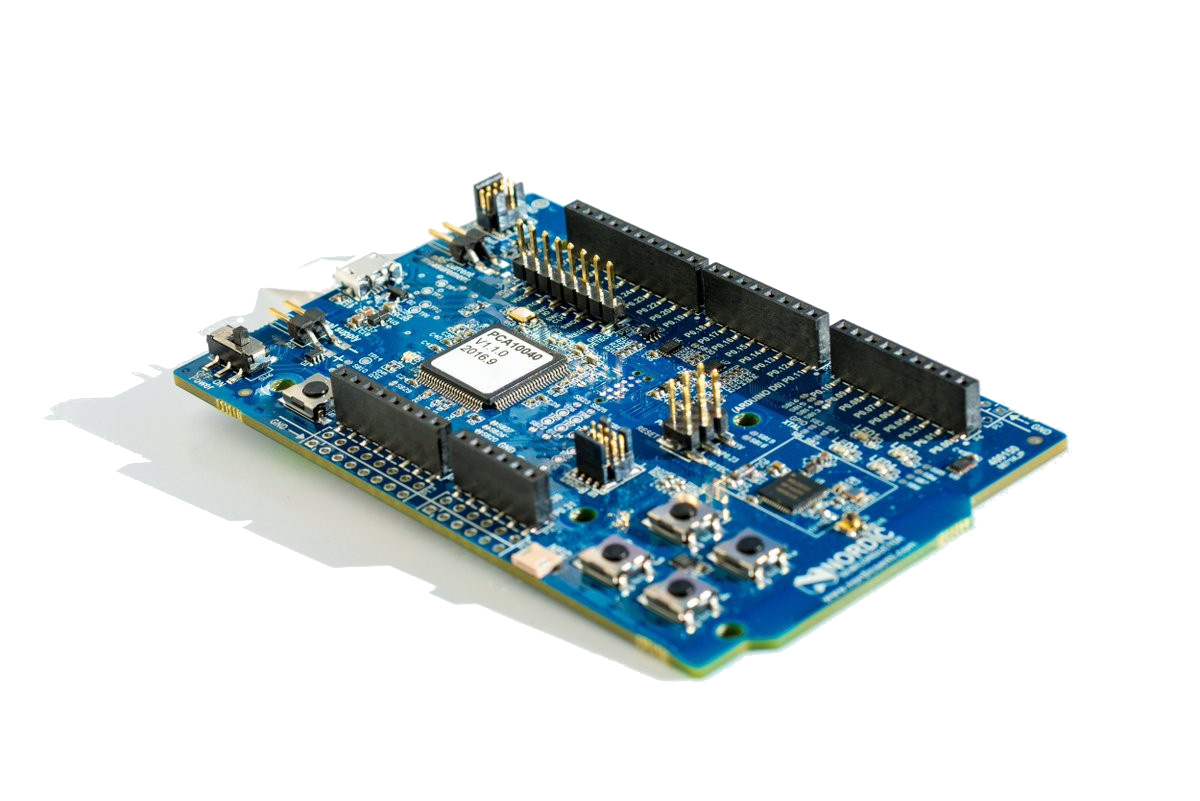
\includegraphics[width=1.0\linewidth]{bilder/nrf52_board.jpg}
	\caption{Das nRF52 Development Kit}
	\label{fig:devkit}
\end{figure}

Das nRF52 DK ist eine single-Board Entwicklungsplatform welche f�r die Verwendung von \ac{BLE}, ANT, und propriet�ren 2.4GHz Protokollen ausgelegt ist. Herzst�ck des Kits ist das nRF52832 \ac{SoC}.

Die Header sind kompatibel mit allen Arduino Shields des Revisionsstandards 3 was das Kit enorm erweiterbar macht. Weiter besteht die M�glichkeit eine mitgelieferte NFC-Antenne anzuschliessen um NFC-Tags zu lesen. Alle GPIOs sind via Header herausgef�hrt. Zus�tzlich verf�gt das Board �ber 4 LEDs und 4 Taster. 

\newpage

\section{Technische �bersicht}

\begin{figure}[h]
	\centering
	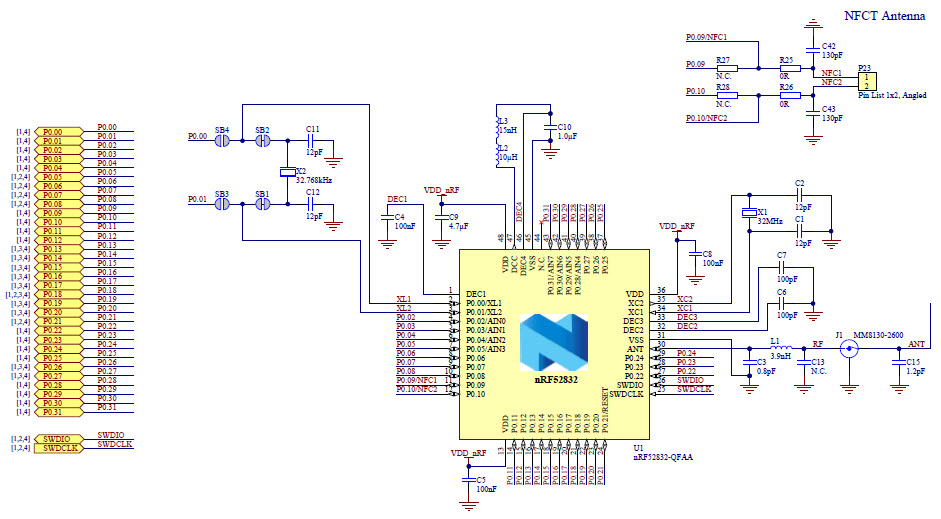
\includegraphics[width=1.0\linewidth]{bilder/nrf52_schematic.jpg}
	\caption{Schema des nRF52DKs aus der Dokumentation von Nordic entnommen}
	\label{fig:schematic}
\end{figure}

\section{Installation der GNU ARM Embedded Toolchain}

Um die Funktion aller Tools und der SDK zu gew�hrleisten, sollten folgende Installationen ausschliesslich in der hier beschriebenen Reihenfolge ausgef�hrt werden. Da sich die Installation unter Ubuntu und Arch Linux unterscheiden, sind im nachfolgenden beide Varianten dokumentiert. 

Um die Software auf dem Hostsystem f�r das nRF52DK kompilieren zu k�nnen, ben�tigen wir eine sogenannte crosscompiler-toolchain. F�r ARM basierte Controller ist hier die erste Wahl die gnu-arm-none-eabi Toolchain. Sie l�sst sich von folgender Seite beziehen:

\url{https://launchpad.net/gcc-arm-embedded/+download}

Es gilt darauf zu achten, die neueste Version zu verwenden und sich zu notieren, welche Version heruntergeladen wurde, da diese sp�ter im Makefile angegeben werden muss. Die Software sollte im Verzeichnis /opt installiert werden. Die Binaries sollten mit den n�tigen Rechten ausgestattet werden. Weiter empfiehlt es sich symbolische Links zu generieren, um die Programme systemweit sichtbar zu machen.

Die Befehle dazu lauten:

\begin{lstlisting}[style=BashInputStyle]
    tar -xf gcc-arm-none-eabi-linux.tar.bz2 /opt/gcc-arm-none-eabi-tools
    ln -s /opt/gcc-arm-none-eabi-tools/bin/* /usr/local/bin/
\end{lstlisting}

Wichtig: Unter Arch Linux sollte unbedingt die aktuellste Version im Community Repository verwendet werden. Die gew�nschte Software l�sst sich wie folgt installieren:

\begin{lstlisting}[style=BashInputStyle]
    pacman -S community/arm-none-eabi-binutils
    pacman -S community/arm-none-eabi-newlib
    pacman -S community/arm-none-eabi-gcc
    pacman -S community/arm-none-eabi-gdb
\end{lstlisting}


\section{Installation der nordic SDK}

Nordic Semiconductor verf�gt �ber ein Software Archiv von welchem alle ben�tigte Software bezogen werden kann. Das Archiv befindet sich unter folgendem Link:

\url{https://www.nordicsemi.com/eng/Products/Bluetooth-low-energy/nRF52-DK#Downloads}

Um mit dem nRF52 Entwicklungskit arbeiten zu k�nnen, ben�tigen wir folgende Softwarepakete:

\begin{enumerate}
    \item nRF5 SDK Zip File
    \item nRF5x-Command-Line-Tools-Linux64
\end{enumerate}

Im ersten Paket befinden sich alle Files, welche zur Entwicklung von Software auf dem nRF52dk notwendig sind. Darunter Makefiles, Linkerskripte und auch Beispielcode.
Im zweiten Paket befinden sich die Command-Line-Tools, welche es uns erm�glichen �ber die Kommandozeile mit dem nRF52 Entwicklungskit zu kommunizieren. Das wichtigste Tool ist nrfjprog, welches kompilierte Programme auf das Board hochladen kann.

Die SDK sowie die Command-Line-Tools sollten auf dem System unter dem Ordner /opt installiert werden und mit den n�tigen Berechtigungen versehen werden. Ebenfalls sollten die Programme in einen Ordner gelinkt werden, welcher im Systempfad angegeben ist.

Die Befehle dazu lauten:
\begin{lstlisting}[style=BashInputStyle]
    tar -xf nRF5x-Command-Line-Tools-Linux64.tar /opt/
    ln -s /opt/nrfjprog/nrfjprog /usr/bin/nrfjprog
    ln -s /opt/mergehex/mergehex /usr/bin/mergehex
\end{lstlisting}

Unter Arch Linux lassen sich die Command Line Tools auch �ber das Arch User Repository beziehen. Dazu kann man den Pacman Wrapper ''yaourt'' verwenden:

\begin{lstlisting}[style=BashInputStyle]
    yaourt -S aur/nrf5x-command-line-tools 
\end{lstlisting}

\section{Installation des SEGGER JLink Debuggers}

Die Software von SEGGER, welche f�rs Debuggen gebraucht wird, findet man unter folgendem Link:

\url{https://www.segger.com/downloads/jlink}

Das Paket ''J-Link Software and Documentation Pack'' enth�lt verschiedene Programme. Die Wichtigsten davon sind der JLinkCommander und der JLinkGDBServer. �ber den Commander l�sst sich die CPU des nRF52 vollst�ndig via JTAG oder SWD Schnittstelle kontrollieren. Der JLinkGDBServer stellt auf dem Localhost einen Socket unter Port 2331 zur Verf�gung, auf welchen man sich mit GDB verbinden kann.

Die JLink Toolchain sollte auf dem System unter dem Ordner /opt installiert werden und mit den n�tigen Berechtigungen versehen werden. Die Programme sollten mittels symbolischen Links in einen Ordner gelinkt werden, welcher im Systempfad angegeben ist.

\begin{lstlisting}[style=BashInputStyle]
    mkdir /opt/SEGGER/JLink
    tar -xzf JLink_Linux_{VERSION}.tar.gz /opt/SEGGER/JLink
    ln -s /opt/SEGGER/JLink/JLinkExe /usr/bin/JLinkExe
    ln -s /opt/SEGGER/JLink/JLinkGDBServer /usr/bin/JLinkGDBServer
\end{lstlisting}

SEGGER bietet auch ein Debianpaket an. Dieses kann auf Systemen, welche �ber den Paketmanager DPKG verf�gen mittels \verb|dpkg -i JLink_linux.deb| installiert werden. Dadurch entf�llt obiger Installationsaufwand.\newline

Unter ArchLinux l�sst sich die Software auch aus dem Arch-User-Repository installieren, der Befehl dazu lautet:
\begin{lstlisting}[style=BashInputStyle]
    yaourt -S aur/jlink-software-and-documentation
\end{lstlisting}

\section{Verwendung des JLinkGDBServers}

Der folgende Befehl beschreibt das Starten des GDBJLinkServers von SEGGER. 

\begin{lstlisting}[style=BashInputStyle]
    JLinkGDBServer -Device nRF52832_xxAA -If SWD -Speed 4000 -Autoconnect 1
\end{lstlisting}

Der Server startet einen lokalen Socket und ist unter Port 1234 erreichbar.
Nachdem \ac{GDB} gestartet wurde, l�sst sich �ber folgenden Befehl eine Verbindung mit dem Server herstellen:

\textbf{(gdb) target remote localhost:1234}

Alternativ kann auch eine Konfigurationsdatei f�r GDB angelegt werden. Dazu erstellt man im Home-Verzeichnis eine Datei mit dem Namen .gdbinit. Um automatisch auf den lokalen Server zu verbinden ist lediglich die obere Zeile hinzuf�gen. 

\section{Verwendung von nrfjprog}

Nrfjprog ist Teil der Propriet�ren Softwarewerkzeuge der SDK von Nordic. Es unterst�tzt das Flashen von Hex-Binarys �ber SWD oder JTAG. Der Funktionsumfang ist sehr gross, daher sei an dieser Stelle auch noch aufs Helpfile verwiesen.

Um eine bereits kompilierte Beispielapplikation auf das nrf52 Board zu laden sind folgende Befehle in dieser Reihenfolge auszuf�hren.

\begin{lstlisting}[style=BashInputStyle]
    nrfjprog --eraseall -f nrf52
    nrfjprog --program outdir/nrf52_pca10040/zephyr.hex -f nrf52
    nrfjprog --reset -f nrf52
\end{lstlisting}

Zeile 1 l�scht den aktuellen Inhalt des Flashspeichers auf dem SoC.\newline
Zeile 2 flasht ein neues Binary in den Flashspeicher des SoC.\newline
Zeile 3 Resetet den SoC, alternativ kann auch der Hardwarereset bet�tigt werden.\newline

% !TeX encoding = ISO-8859-1
\chapter{DemoApp}
\label{chap:demoapp}

\section{Technische �bersicht}
\section{Hardware Dokumentation}
\section{Software Dokumentation}
\section{Softwaretests}
% !TeX encoding = ISO-8859-1
\chapter{Fazit}
\label{chap:fazit}

\section{Vergleich Ist/Soll}

Wir sind mit dem erreichten Resultat zufrieden. Unsere Arbeit bietet einen horizontalen �berblick �ber das Zephyr-Betriebssystem. Ausserdem konnte ein detaillierter Beschrieb des Aufbaus und der Ziele des Betriebssystems erl�utert werden. Zudem wird ein �berblick �ber einige technische Details, wie z.B. Technologien, Protokolle und Anwendungen gew�hrt. Im Vergleich zu anderen Berichten, sofern diese schon vorliegen in diesem Bereich, konnten wir unser Ziel, eine umfassendere Zusammenfassung der wichtigsten Protokolle und Anwendungsprobleme bieten, damit Forscher und Anwendungsentwickler einen schnellen �berblick �ber die gew�nschten Funktionalit�ten erhalten. 

Ein weiteres Ziel das wir uns f�r die Projektarbeit gestellt haben ist die Entwicklung einer Demonstrationsapplikation f�r Zephyr, welche als Beispielprojekt f�r Neuentwicklungen dienen kann. Im Verlaufe der Projektarbeit musste das Pflichtenheft dieser Demoapp leider abgespeckt werden. Das Zephyr-OS war zur Zeit der Durchf�hrung der Projektarbeit noch unter aktiver Entwicklung. Auch die Unterst�tzung des nRF52 Development Kits beschr�nkte sich gr�sstenteils auf Bluetooth und Wireless. Die Dokumentation aller weiteren Funktionalit�ten f�r das Board war noch nicht vorhanden, was Entwicklungsarbeiten enorm erschwerte. Die Ursache ist damit zu begr�nden, dass das Board wegen der propriet�ren Toolchain vom Buildsystem noch nicht vollst�ndig unterst�tzt ist. Das bedeutet, dass zur Entwicklung Tools wie die Eclipse IDE nur beschr�nkt einsetzbar sind.
Im Rahmen der Projektarbeit haben wir daher ein Shellscript geschrieben welche die oben genannten Funktionalit�ten mit bringt. Eine Anpassung des Makefiles des Zephyr Build-Systems w�re w�nschenswert und w�rde den Support der Produktepalette von Nordic ganz sicher vorantreiben. Dies h�tte jedoch den von uns gesteckten Rahmen der Arbeit gesprengt, daher haben wir uns auf die Entwicklung des Shellscripts begrenzt.
Als Demonstrationsapplikation dient momentan das Eddystone Beacon Example des Zephyrprojektes. Das Beispielprogramm wurde jedoch f�rs nRF52 Board angepasst und in ein eigenes Projekt umgewandelt. Weiter entwickelten wir eine "Hello World" Applikation welche vom nrf52dk-zephyr-tool beim Anlegen eines neuen Projektes generiert wird. Diese Applikation zeigt die Verwendung der GPIOs des Boards. 
Die gesammelten Erfahrungen k�nnen in sp�teren Projekten der Berner Fachhochschule bestimmt gut gebraucht werden. Als Schlussbetrachtung kann gesagt werden, dass das Projekt eine gewisse Herausforderung war. Viele Teile des Zephyr-Projektes sind noch nicht Dokumentiert und es bedurfte bis zu einem gewissen Grad Reverse Engineering und Trial-And-Error um beispielsweise die richtigen Kernelkonfigurationen zu finden, damit die Software auf unserem Board l�uft. Nichtsdestotrotz war es ein sehr interessantes und abwechslungsreiches Projekt. 

Wir m�chten uns hiermit bei unserem Betreuer Herr Martin Aebersold f�r die gute Unterst�tzung bedanken.

\section{W�nschenswerte Erweiterungen}

W�nschenswert w�re sicher die Erweiterung des Makefiles um das nRF52 Board besser zu unterst�tzen. Weiter sollte man sich vertiefter mit der Entwicklung von Sensortreibern auseinandersetzen. Zephyrs Erfolg h�ngt schlussendlich davon ab wie gut die zur Zeit popul�ren Sensoren und Ger�te unterst�tzt werden.   
Je mehr Support, desto weiter wird sich das RTOS verbreiten k�nnen. Hier sehen wir auch grosse Chancen f�r die Open-Source Entwicklung. Nachfolgende Projekte k�nnten sich beispielsweise mit der Entwicklung eines Treiber besch�ftigen. 

Auch die Portierung des Zephyr Kernels auf ein andere Plattform wie beispielsweise das ESP8266 w�re ein Interessantes Thema f�r ein Folgeprojekt. 


%---------------------------------------------------------------------------

% Selbst�ndigkeitserkl�rung
%---------------------------------------------------------------------------
\cleardoublepage
\phantomsection 
\addcontentsline{toc}{chapter}{Selbst�ndigkeitserkl�rung}
\chapter*{Selbst�ndigkeitserkl�rung}
\label{chap:selbstaendigkeitserklaerung}

\vspace*{10mm} 

Ich/wir best�tige/n, dass ich/wir die vorliegende Arbeit selbstst�ndig und ohne Benutzung anderer als der im Literaturverzeichnis angegebenen Quellen und Hilfsmittel angefertigt habe/n. S�mtliche Textstellen, die nicht von mir/uns stammen, sind als Zitate gekennzeichnet und mit dem genauen Hinweis auf ihre Herkunft versehen. 

\vspace{15mm}

\begin{tabbing}
xxxxxxxxxxxxxxxxxxxxxxxxx\=xxxxxxxxxxxxxxxxxxxxxxxxxxxxxx\=xxxxxxxxxxxxxxxxxxxxxxxxxxxxxx\kill
Ort, Datum:		\> [Biel/Burgdorf], \versiondate \\ \\ 
Namen Vornamen:	\> [Test Peter] 	\> [M�ster R�s�] \\ \\ \\ \\ 
Unterschriften:	\> ......................................\> ...................................... \\
\end{tabbing}

%---------------------------------------------------------------------------

% Glossary
%---------------------------------------------------------------------------
\phantomsection 
\addcontentsline{toc}{chapter}{Glossar}

\newglossaryentry{BibTeX}{name={BibTeX},description={Programm zur Erstellung von Literaturangaben und -verzeichnissen in \TeX- oder \LaTeX-Dokumenten}}
\newglossaryentry{StwVrz}{name={Stichwortverzeichnis},description={Verzeichnis mit Stichworten aus dem Text}}



%\printglossary
%---------------------------------------------------------------------------

% Bibliography
%---------------------------------------------------------------------------
\cleardoublepage
\phantomsection 
\addcontentsline{toc}{chapter}{Literaturverzeichnis}
\bibliographystyle{IEEEtranS}
\bibliography{datenbanken/bibliography}{}
%---------------------------------------------------------------------------

% Listings
%---------------------------------------------------------------------------
\cleardoublepage
\phantomsection 
\addcontentsline{toc}{chapter}{Abbildungsverzeichnis}
\listoffigures
\cleardoublepage
\phantomsection 
\addcontentsline{toc}{chapter}{Tabellenverzeichnis}
\listoftables
%---------------------------------------------------------------------------

% Index
%---------------------------------------------------------------------------
\cleardoublepage
\phantomsection 
\addcontentsline{toc}{chapter}{Stichwortverzeichnis}
\renewcommand{\indexname}{Stichwortverzeichnis}
\printindex
%---------------------------------------------------------------------------

% Attachment:
%---------------------------------------------------------------------------
\appendix
\settocdepth{section}
\chapter{Beliebiger Anhang}
\label{chap:bel_anhang}

Phasellus eget velit massa, sed faucibus nisi. Etiam tincidunt libero viverra lorem bibendum ut rutrum nisi volutpat. Donec non quam vitae lacus egestas suscipit at eu nisi. Maecenas non orci risus, at egestas tellus. Vivamus quis est pretium mauris fermentum consectetur. Cras non dolor vitae nulla molestie facilisis. Aliquam euismod nisl eget risus pretium non suscipit nulla feugiat. Nam in tortor sapien. Nam lectus nibh, laoreet eu ultrices nec, consequat nec sem. Nulla leo turpis, suscipit in vulputate a, dapibus molestie quam. Vestibulum pretium, purus sed suscipit tempus, turpis purus fermentum diam, id cursus enim mi a tortor. Proin imperdiet varius pellentesque. Nam congue, enim sit amet iaculis venenatis, dui neque ornare purus, laoreet porttitor nunc justo vel velit. Suspendisse potenti. Nulla facilisi.

\chapter{Weiterer Anhang}
\label{chap:anhang_B}

\section{Test 1}
Phasellus eget velit massa, sed faucibus nisi. Etiam tincidunt libero viverra lorem bibendum ut rutrum nisi volutpat. Donec non quam vitae lacus egestas suscipit at eu nisi. Maecenas non orci risus, at egestas tellus. Vivamus quis est pretium mauris fermentum consectetur. Cras non dolor vitae nulla molestie facilisis. Aliquam euismod nisl eget risus pretium non suscipit nulla feugiat. Nam in tortor sapien. 

\subsection{Umfeld}
Nam lectus nibh, laoreet eu ultrices nec, consequat nec sem. Nulla leo turpis, suscipit in vulputate a, dapibus molestie quam. Vestibulum pretium, purus sed suscipit tempus, turpis purus fermentum diam, id cursus enim mi a tortor. Proin imperdiet varius pellentesque. Nam congue, enim sit amet iaculis venenatis, dui neque ornare purus, laoreet porttitor nunc justo vel velit. Suspendisse potenti. Nulla facilisi.

%---------------------------------------------------------------------------

\end{document}

